\begin{frame}
	\frametitle{Steady State Case}
		\textbf{Steady state neutron flux (with \gls{DNP} drift)}
		\begin{columns}
			\column{5cm}
			\begin{figure}
				\centering
				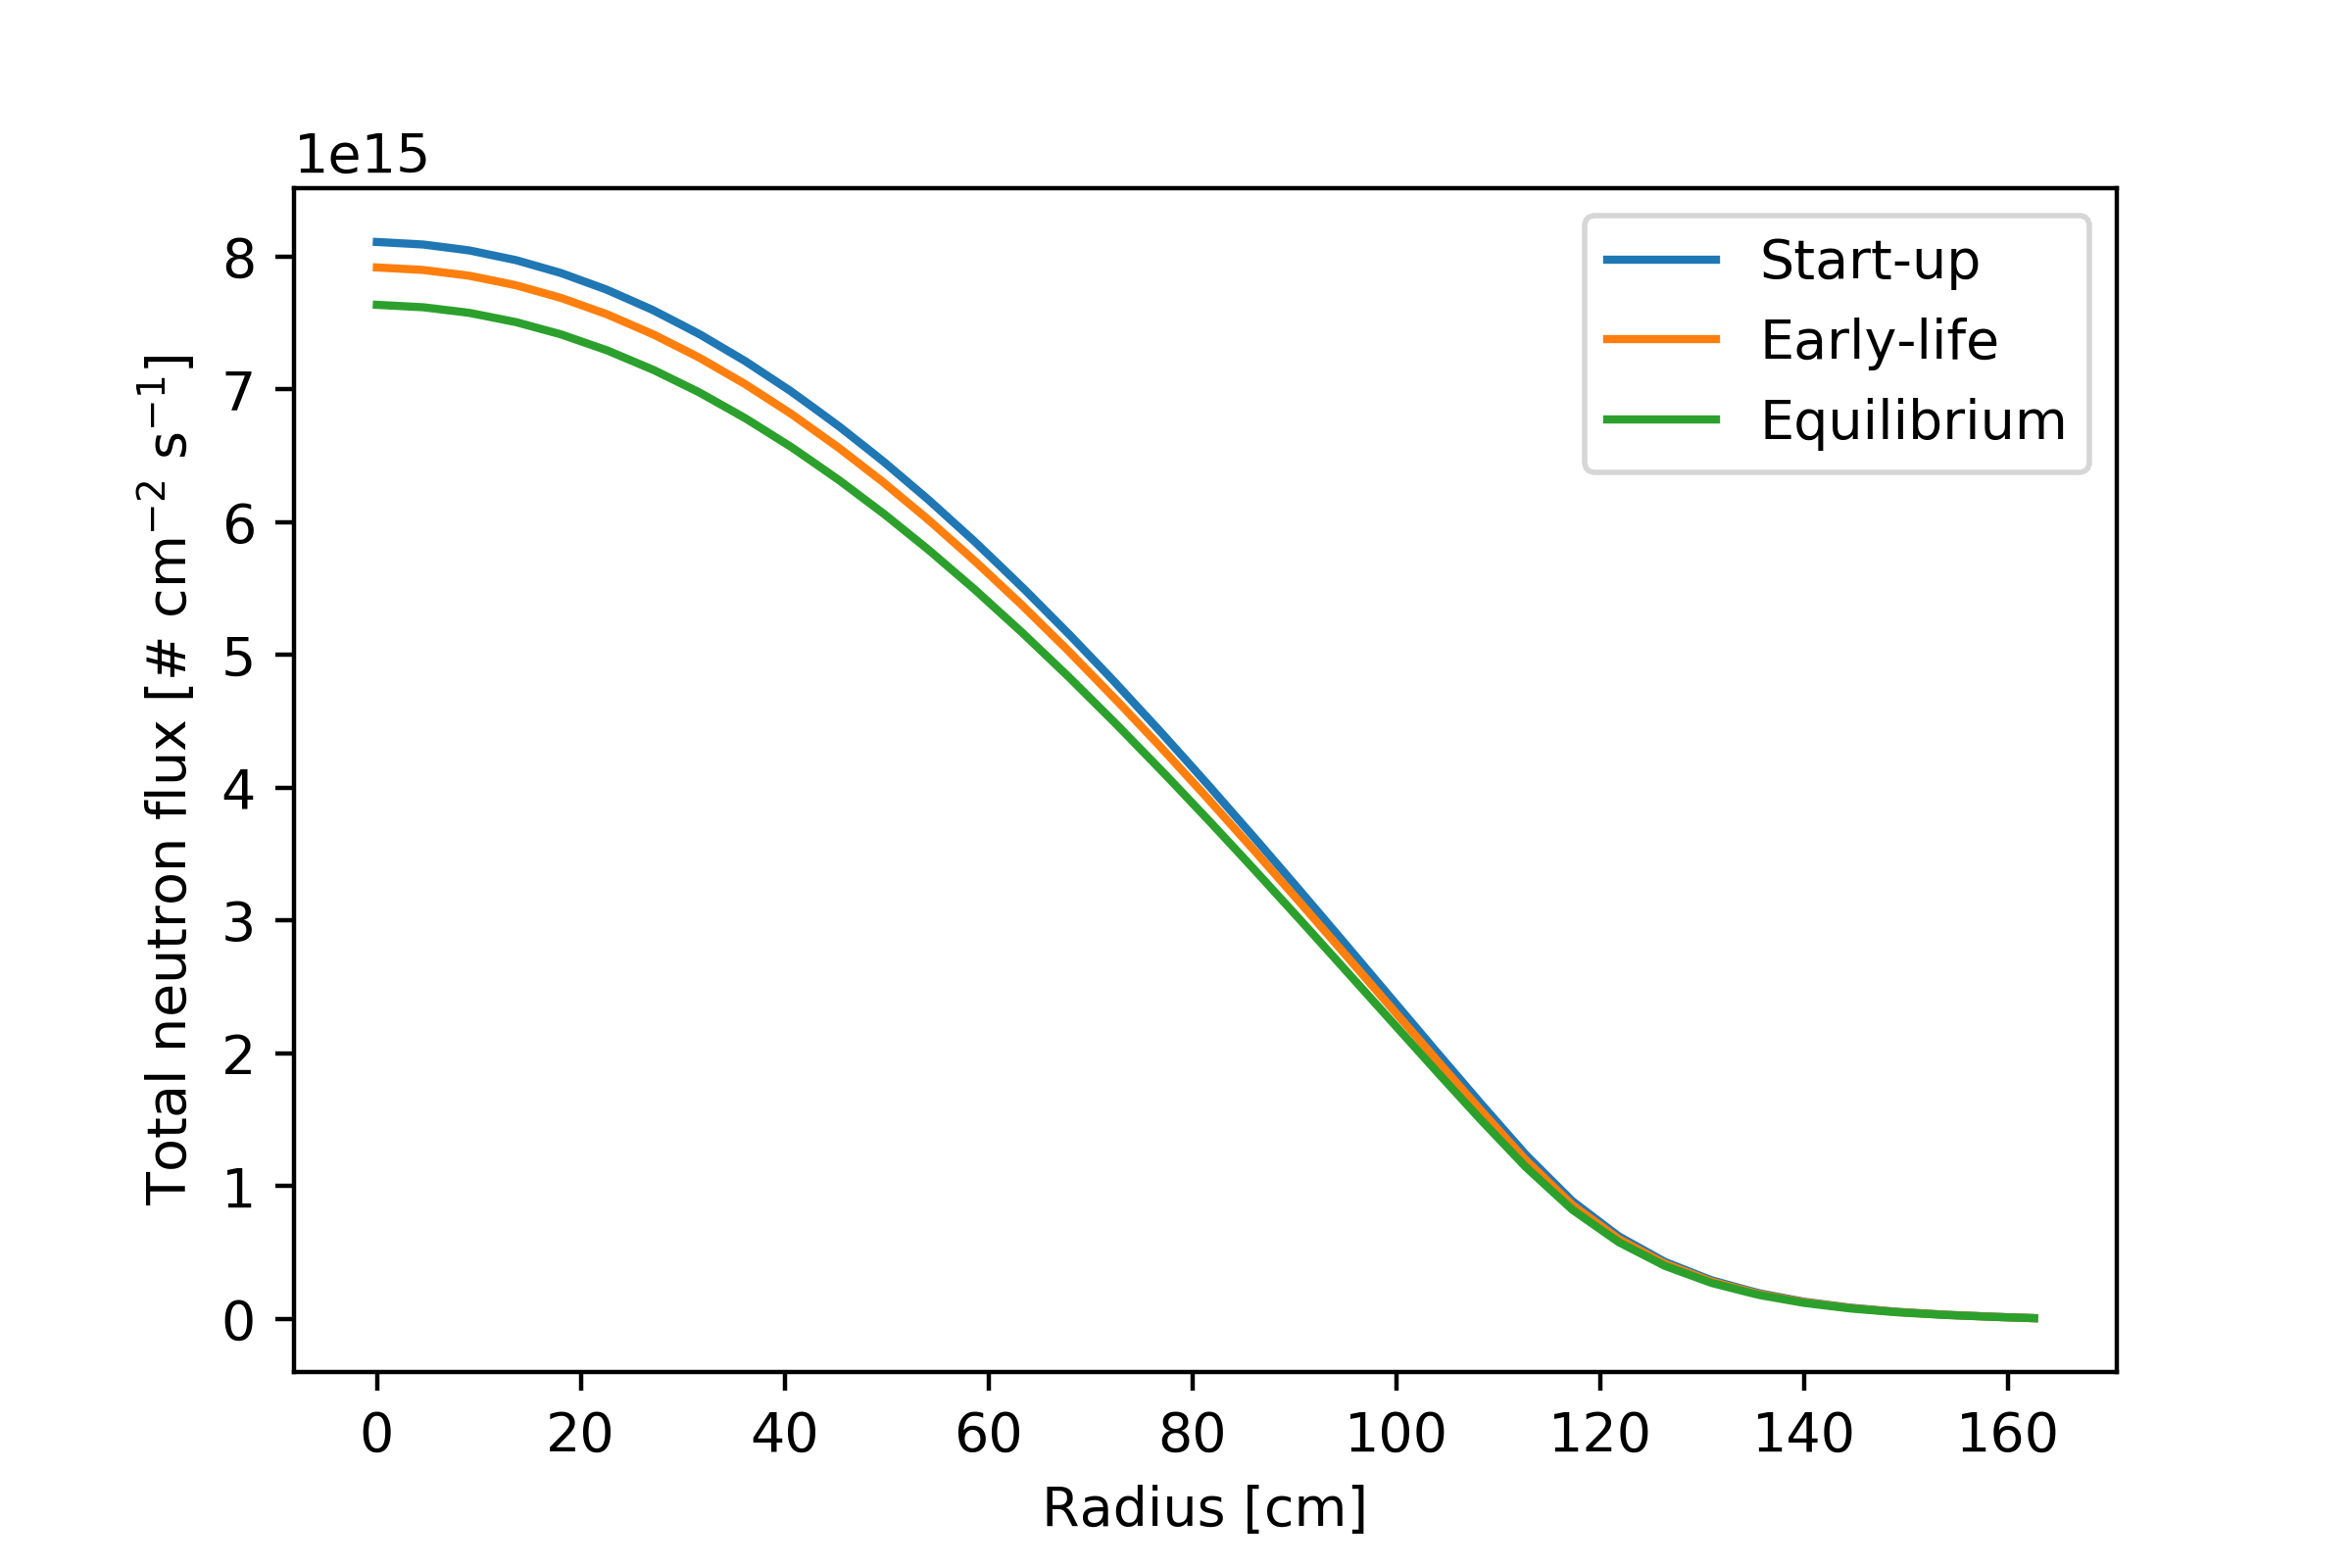
\includegraphics[width=\textwidth]{../paper/figures/totalflux}
				\caption{\small Total radial neutron flux at reactor
				half-height, for start-up, early-life, and equilibrium fuel
				compositions.}
				\label{fig:totalflux}
			\end{figure}
			\column{5cm}
			\begin{figure}
				\centering
				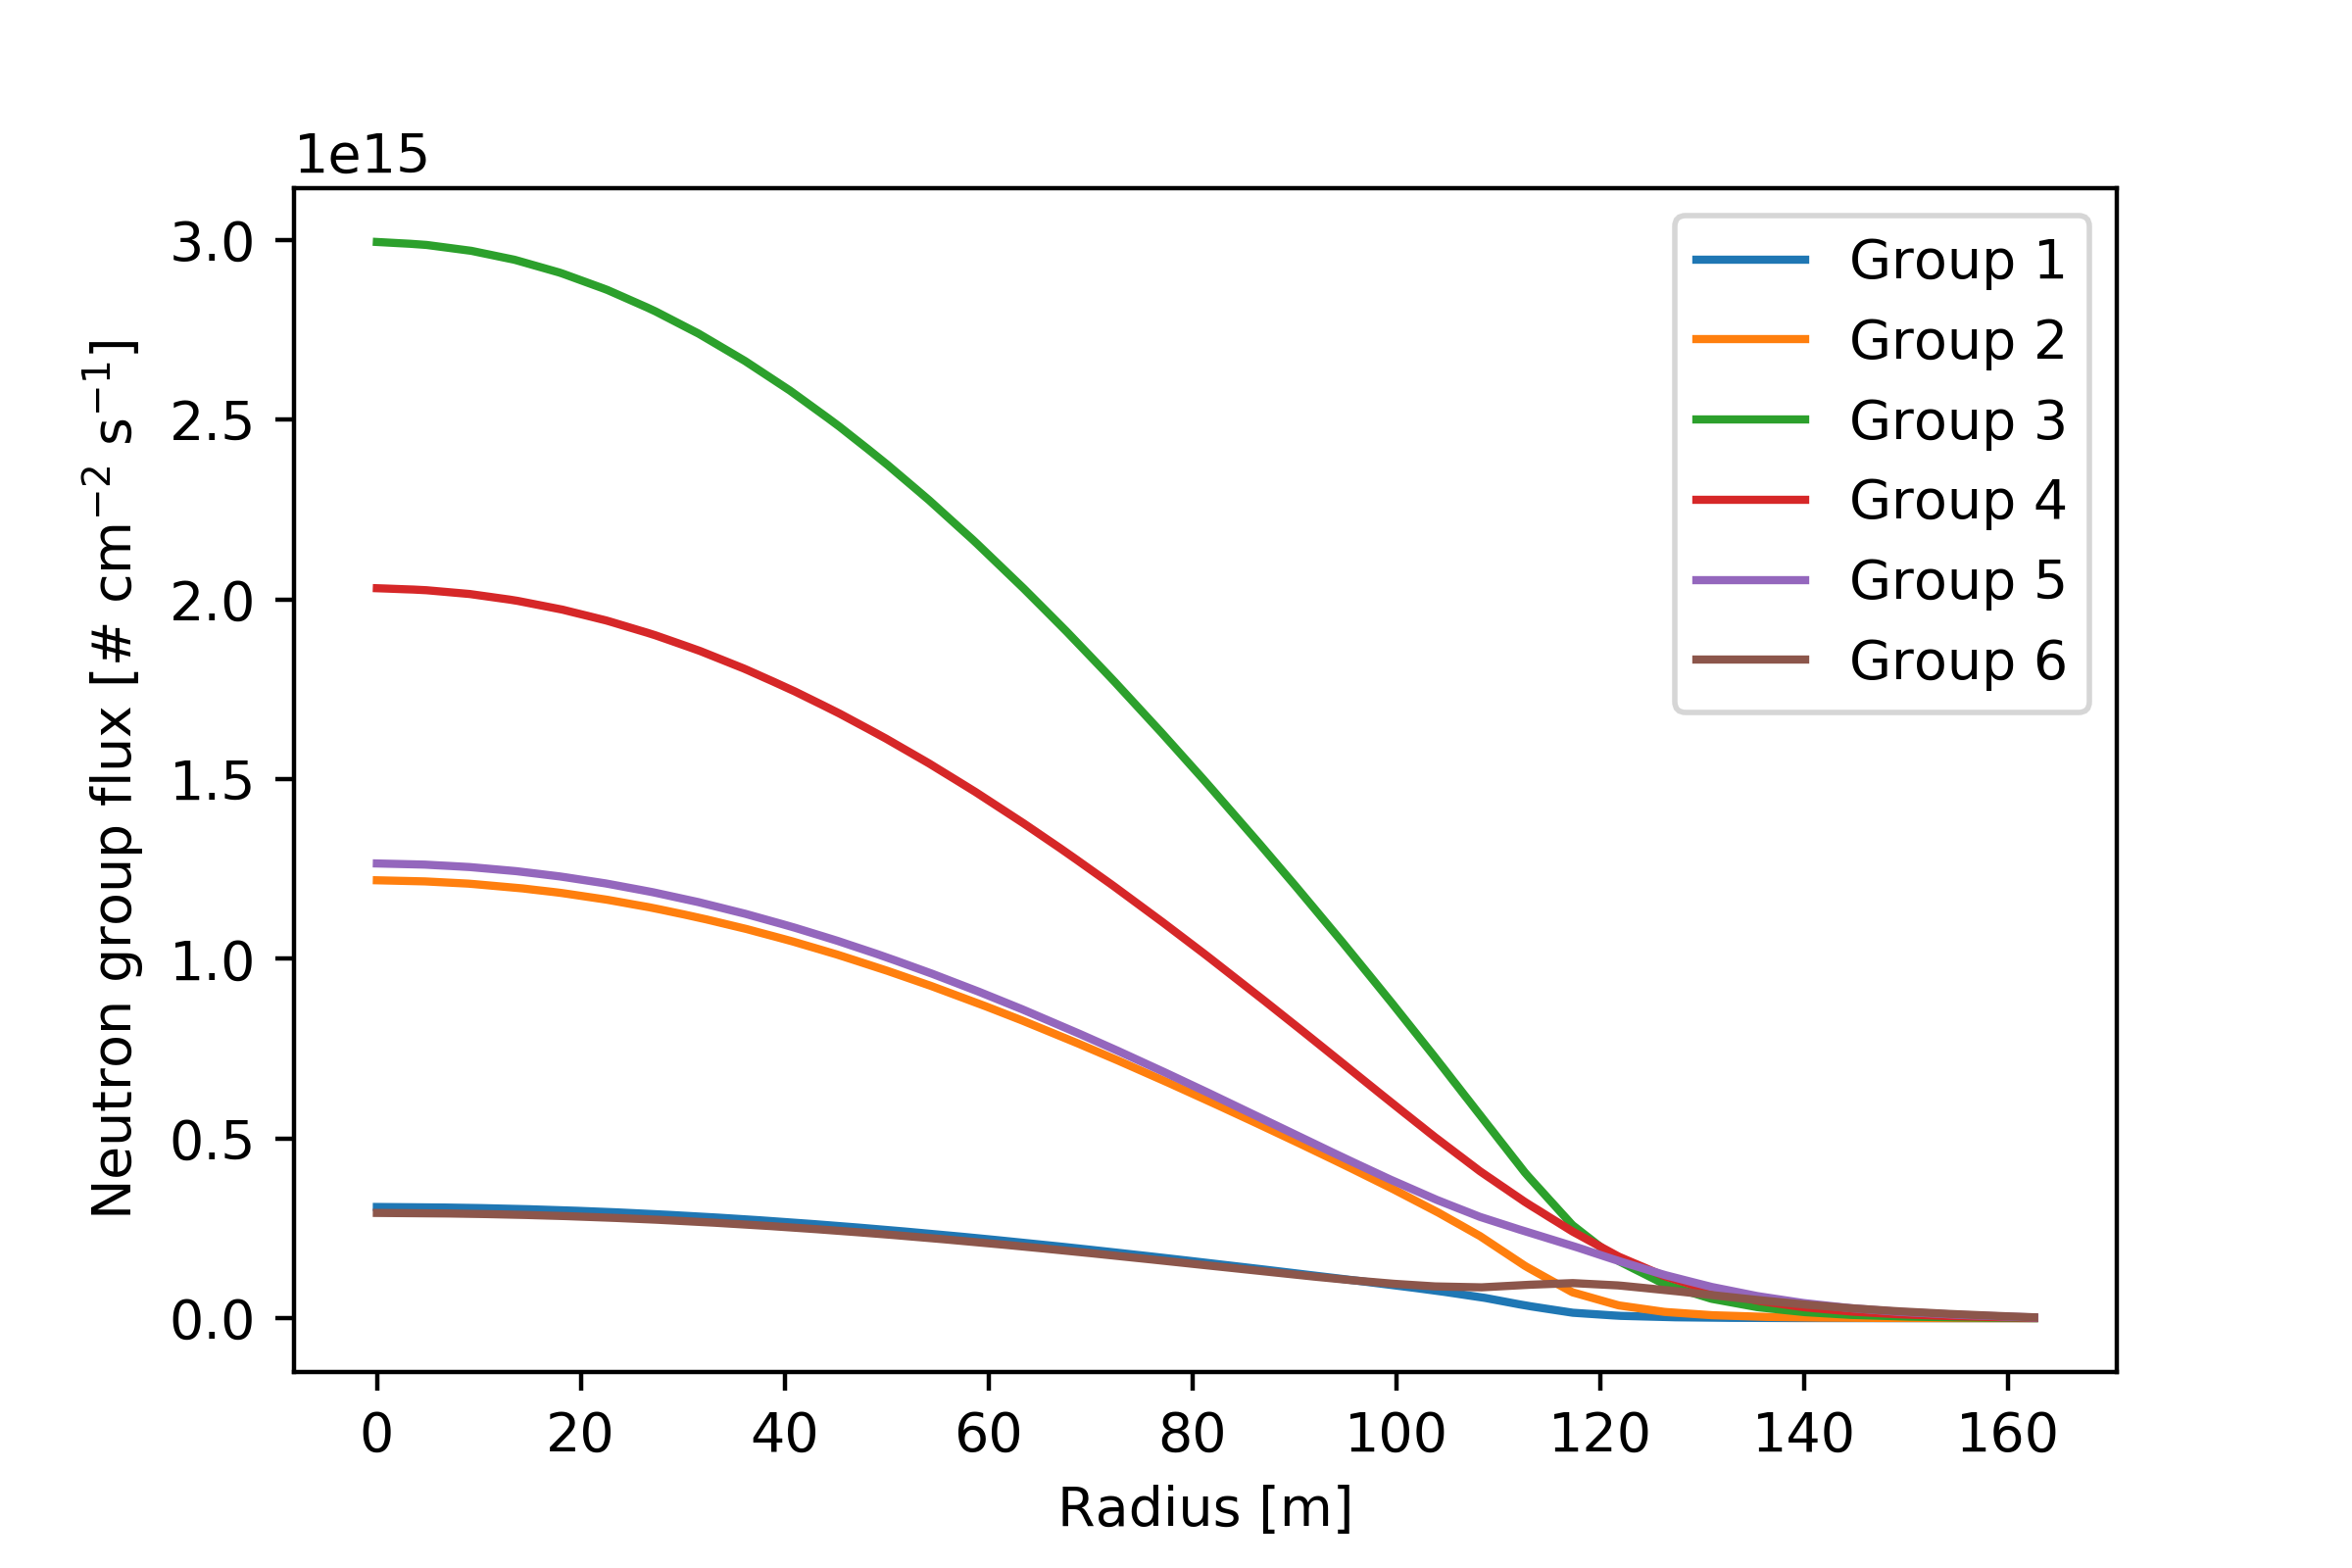
\includegraphics[width=\textwidth]{../paper/figures/stflux}
				\caption{\small Neutron group fluxes at reactor half-height, for
				start-up, early-life, and equilibrium fuel compositions.}
				\label{fig:stflux}
			\end{figure}
		\end{columns}
\end{frame}

\begin{frame}
	\frametitle{Steady State Case}
		\textbf{Steady state temperature distribution}
		\begin{columns}
			\column{12cm}
			\begin{figure}
				\centering
				\begin{subfigure}
					\centering
					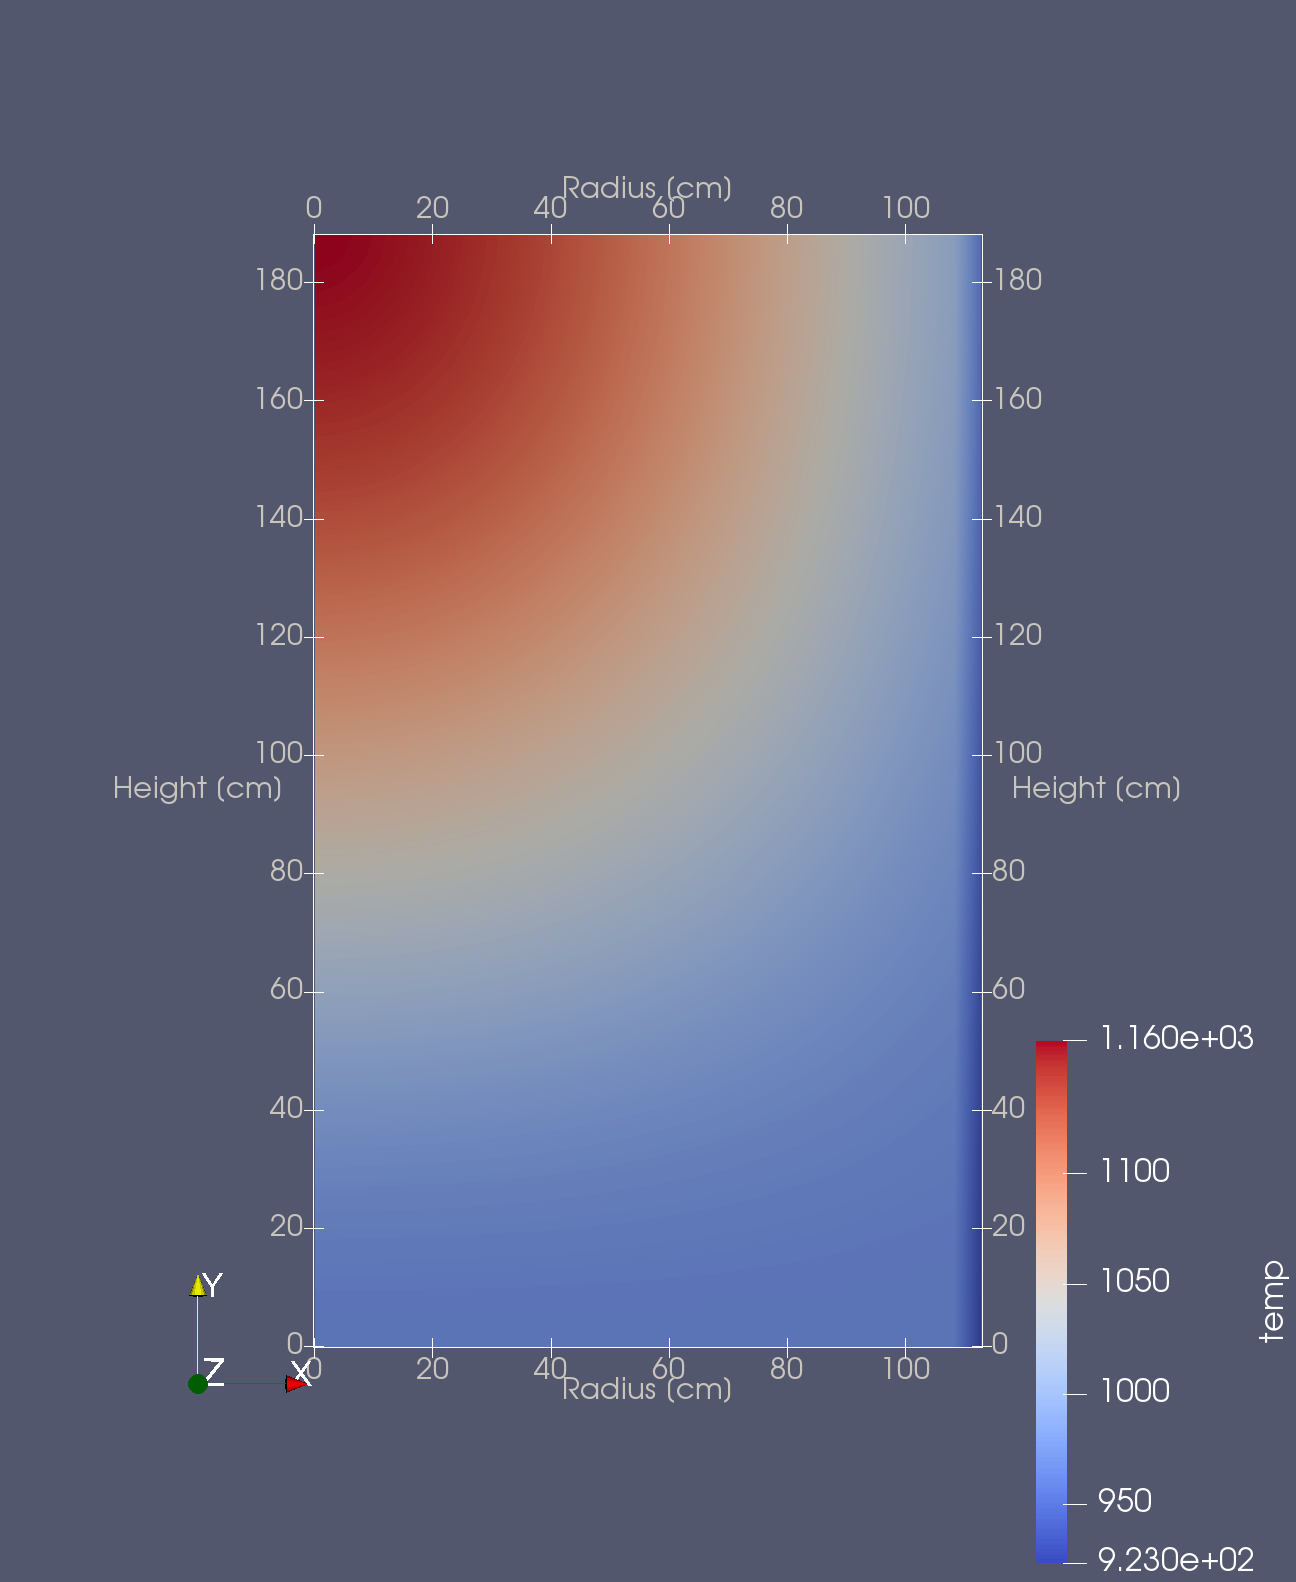
\includegraphics[width=.3\textwidth]{../paper/figures/sttemp}
				\end{subfigure}
				\begin{subfigure}
					\centering
					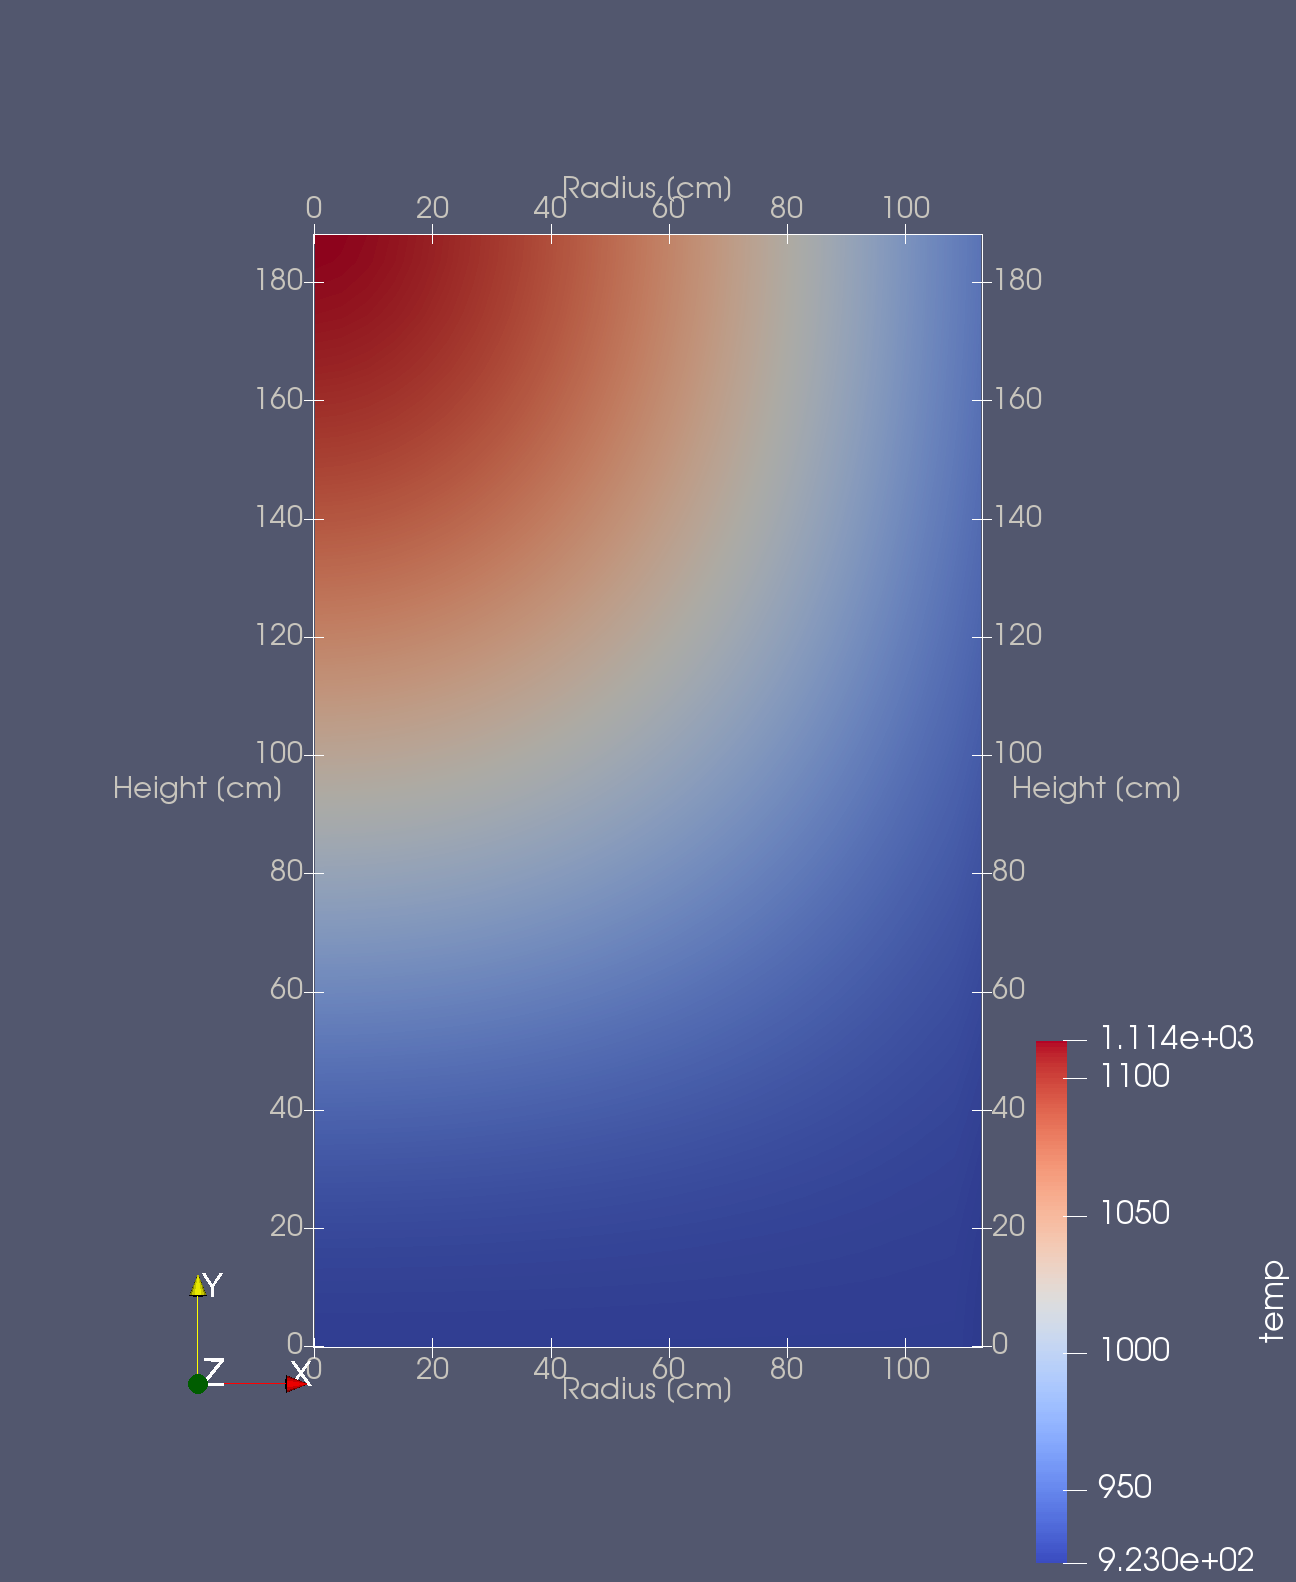
\includegraphics[width=.3\textwidth]{../paper/figures/eltemp}
				\end{subfigure}
				\begin{subfigure}
					\centering
					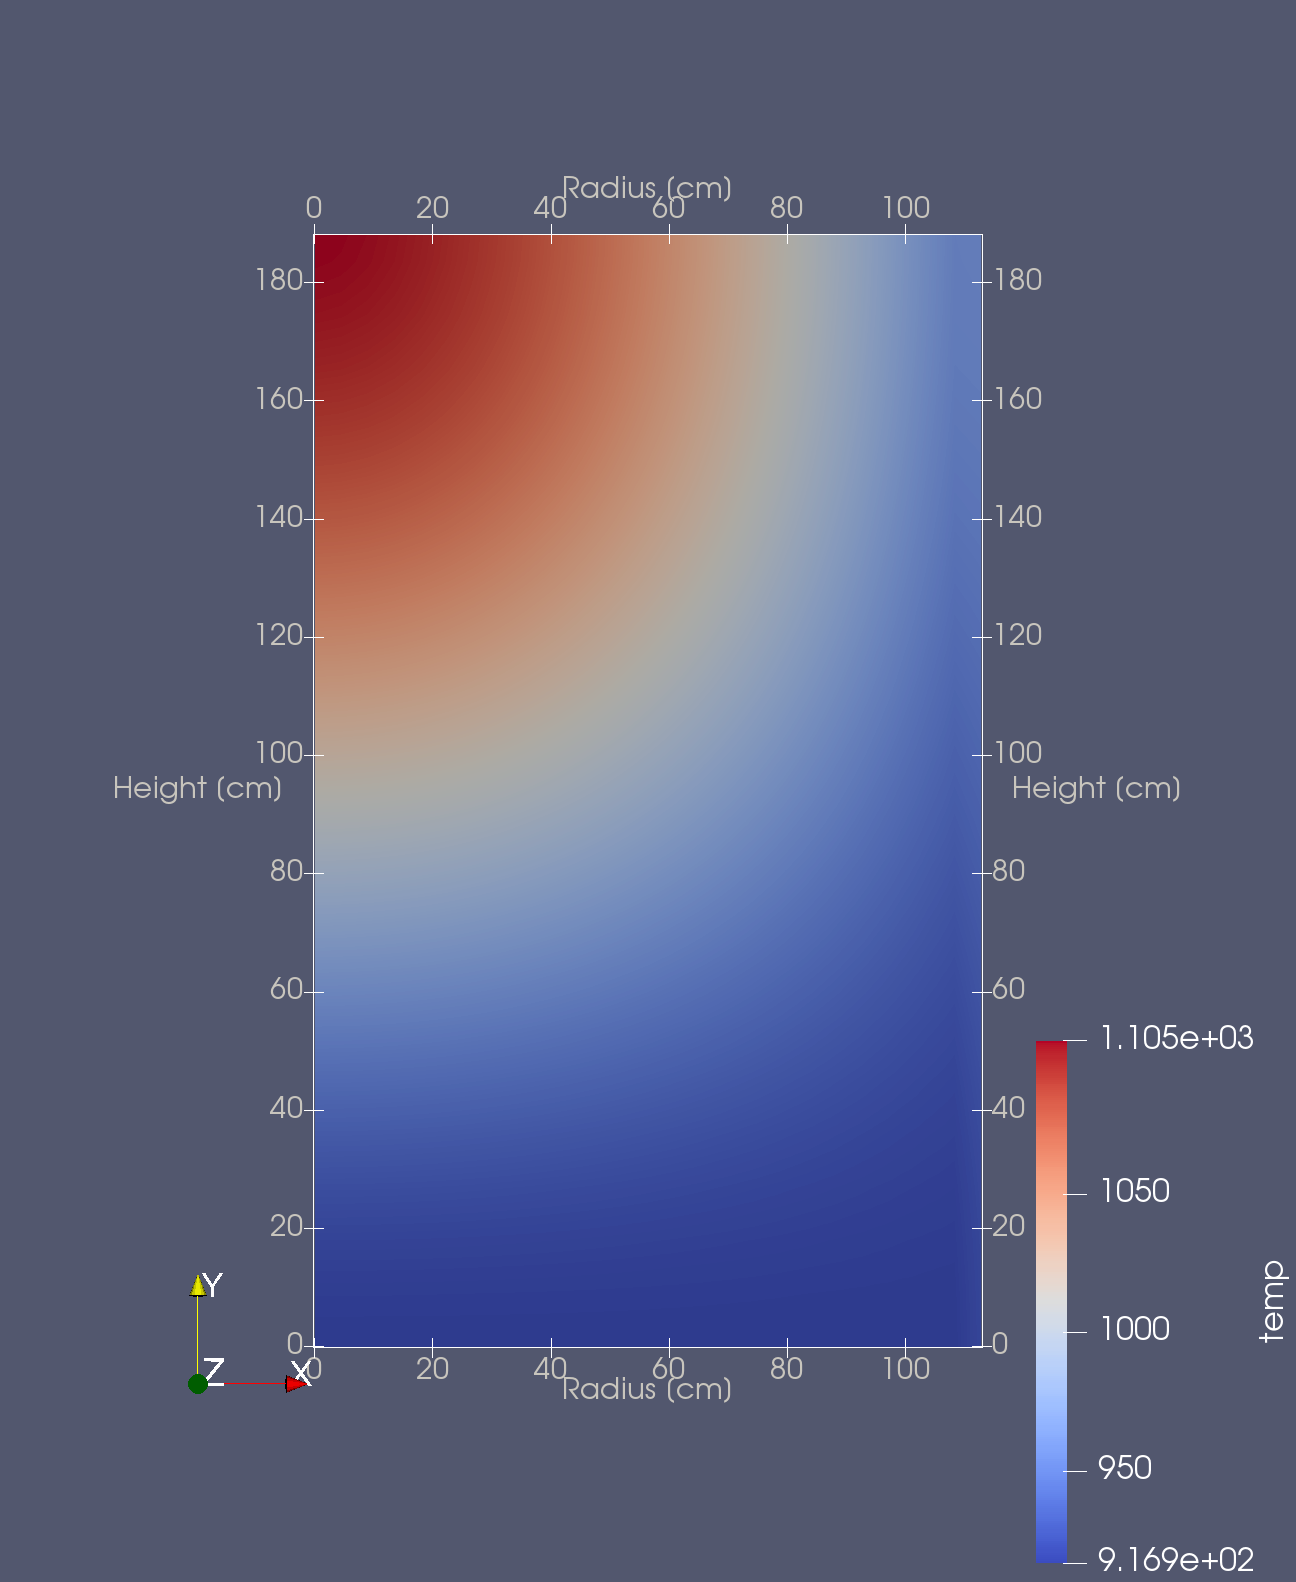
\includegraphics[width=.3\textwidth]{../paper/figures/eqtemp}
				\end{subfigure}\\
				\hspace*{\fill}
				(a) Start-up \hfill \hfill (b) Early-life \hfill \hfill
				(c) Equilibrium
				\hspace*{\fill}
				\caption{Temperature distribution in fuel salt region for
				start-up, early-life, and equilibrium fuel compositions.}
				\label{fig:temp}
			\end{figure}
		\end{columns}
\end{frame}
